\section{Repères et coordonnées}

\subsection{Repères}

\begin{definition}
  Soint $O$, $I$ et $J$ trois points du plan, non alignés.
  $(O, I, J)$ est appelé \emph{repère} du plan.
\end{definition}

\begin{definition}Soit un repère $(O, I, J)$.
  \begin{itemize}
    \item Si $(OI)$ et $(OJ)$ sont perpendiculaires, le repère est dit \emph{orthogonal}.
    \item Si $OI=OJ=1$ (c'est-à-dire si $OIJ$ est isocèle en $O$, et $OI=1$), le repère est dit \emph{normé}.
    \item Si le repère est orthogonal et normé, il est dit \emph{orthonormé}.
  \end{itemize}
\end{definition}

\begin{remarque}
  En seconde, on utilisera \emph{principalement} des repères orthonormés.
\end{remarque}

\begin{exemple}TODO Exemples de repères normé, orthogonal, orthonormé.
\end{exemple}

\subsection{Coordonnées de points}

\begin{wrapfigure}{r}{0pt}
  \centering
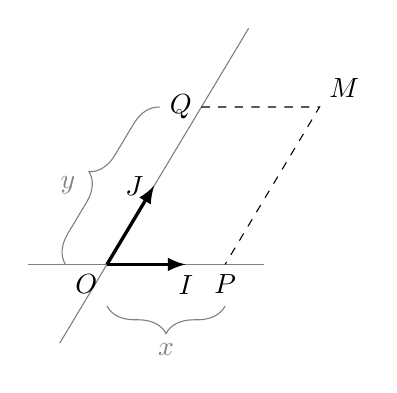
\begin{tikzpicture}[x={(1,0)},y={(.6,1)},>=latex]
    \draw[gray] (-1,0) -- (2,0);
    \draw[gray] (0,-1) -- (0,3);
    \draw[very thick,->] (0,0) -- (1,0) node[below]{$I$};
    \draw[very thick,->] (0,0) -- (0,1) node[left]{$J$};
    \draw (0, 0) node[below left]{$O$};

    \draw[dashed] (0,2) node[left]{$Q$} -- (1.5,2) node[above right]{$M$} -- (1.5,0) node[below]{$P$};

    \draw[decorate,decoration={brace,amplitude=10pt},gray,xshift=-1.5em,yshift=0pt](0,0) -- (0,2) node[midway,left,xshift=-1em]{$y$};
    \draw[decorate,decoration={mirror,brace,amplitude=10pt},gray,yshift=-1.5em,xshift=0pt](0,0) -- (1.5,0) node[midway,below,yshift=-1em]{$x$};
\end{tikzpicture}
\end{wrapfigure}
~

\begin{propriete}
  Soit $(O, I, J)$ un repère du plan, et $M$ un point. Ce point est repéré par un unique couple, appelé
  \emph{coordonnées} de $M$ dans le repère $(O, I, J)$.
\end{propriete}

\begin{remarque}
  Une définition rigoureuse des \emph{coordonnées} sera donnée dans
  le chapitre \emph{Vecteurs}.
\end{remarque}

\section{Propriétés}

\begin{propriete}
  Soient $A(x_A,y_A)$, $B(x_B,y_B)$, $I(x_I,y_I)$ trois point du plan. Alors $I$ est le milieu de $[AB]$ si et seulement si $x_I=\frac{x_A+x_B}{2}$ et $y_I=\frac{y_A+y_B}{2}$.
\end{propriete}

\begin{propriete}
  Soient $A(x_A,y_A)$ et $B(x_B,y_B)$ deux points du plan muni d'un repère orthonormé. Alors la longueur $AB$ est égale à $\sqrt{\left(x_B-x_A\right)^2+\left(y_B-y_A\right)^2}$.
\end{propriete}

\section{Triangles particuliers}

TODO

\section{Quadrilatères}

TODO
